\documentclass{article}

% cool tables
\usepackage{booktabs}
\newcommand{\ra}[1]{\renewcommand{\arraystretch}{#1}}

% images
\usepackage{graphicx}


\title{
    \normalsize \textsc{Rock Concert Audience as a Screen}\\
    \Huge Project plan}
\author{Agnethe Soraa,
Tomas Dohnalek,
Jan Bednarik,
Milos Jovac \\
\normalsize Project adviser: Anh Nguyen Duc}
\date{\today}

\begin{document}
\maketitle
\section{Project customer}
Netlight AS is a consulting company engaged in IT and management. They operates throughout Europe with offices in Stockholm, Oslo, London, Munich and Helsinki. The company was founded at 1999 and employs to 500 employees.

\section{Project description}
- PR text
- effects

\section{Required work}
\section{Project scope}


\section{Project architecture}


\section{Measurement of Project Effects}
To measure success of our end-product we have to set up some criteria to be fulfilled. The product should pass all test-cases and function according to customer's requirements.

\section{Planned workload}
Compendium proposed week workload 25 person-hours per week. During our internal meeting we have decided that each member will spend 30 hours per week because our team consists only of 4 members. We agreed on fixed daily working hours so that we could distribute the workload through the whole semester. We will do daily stand-ups according to Scrum methodology.

\section{General Terms}
\subsection{Tools selections}
For Scrum support and issue tracking we use Gravity Tool\footnote{www.gravitydev.com}. 
The tool is right now in Beta but it is free to use and have all features we needed from proposed AgileZen.
For collaboration on Minutes, Project Plan and other documents we use GitHub. This tool was proposed by out customer and it is popular free collaboration tool.
For document editing we agreed on LaTeX.
For group resources and links we use Facebook groups and for managing shedule we use Google Calendar.
 
\subsection{Limitations}
We should develop this project under a few technical, resource, time and knowlage limitations. 
Big limitation is image processing and small expirience in Mobile development.
As this course last for a 13 weeks, it is normal that we had to make some trade-offs. We devoted 2 weeks in exploring technologies and possible similar solutions that we can benefit from.
  
  
\section{Schedule}
\subsection{Phases}
\paragraph{Sprint 0 (ends 6th of September)}
\paragraph{Sprint 1 (ends 20th of September)}
\paragraph{Sprint 2 (ends 4th of October)}
\paragraph{Sprint 3 (ends 18th of October)}
\paragraph{Sprint 4 (ends 1st of November)}
\paragraph{Sprint 5 (ends 15th of November)}
\subsection{Gantt chart}

\subsection{Milestones}

\begin{figure}[ht]
\begin{center}
    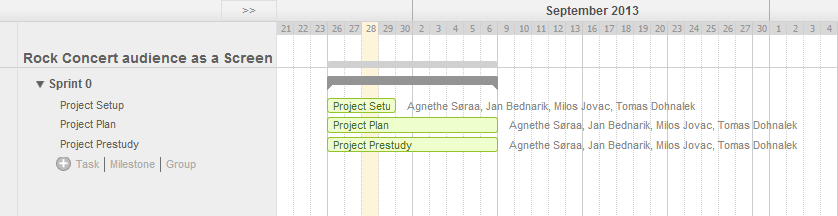
\includegraphics[scale=0.6]{images/gantt}
    \caption{Gantt Chart}
    \label{img:gantt}
\end{center}
\end{figure}
s
\section{Risk management}

\begin{table*}\centering \ra{1.3}
    \caption{Skills}
    \label{tab:skills}
    \vspace{2mm}
    \begin{tabular}{lcccc}
    \toprule
									
    \midrule
    \textbf{Event                	 } & Someone gets sick  		       & 1     & 2     & 3     \\ 
    \textbf{Consiquence              } & 4       					       & 1     & 1     & 1     \\ 
    \textbf{Possibility				 } & 5         						   & 1     & 4     & 1     \\ 
    \textbf{Risk                     } & 20        						   & 4     & 1     & 4     \\ 
    \textbf{Reactive Measures        } & Other people do more ours || Person can work from home         & 3     & 3     & 3     \\ 
    \textbf{Proactive Measures       } & Free weekends        			   & 3     & 1     & 2     \\ 
    \textbf{Responsible              } & All        					   & 2     & 5     & 1     \\ 
   
    \bottomrule
    \end{tabular}
\end{table*}

\begin{table*}\centering \ra{1.3}
    \caption{Skills}
    \label{tab:skills}
    \vspace{2mm}
    \begin{tabular}{lcccc}
    \toprule
                                & Agnethe   & Tomas & Milos & Jan \\
    \midrule
    \textbf{Leadership                 } & 4         & 1     & 2     & 3     \\ 
    \textbf{Scrum                      } & 4         & 1     & 1     & 1     \\ 
    \textbf{Mobile software development} & 3         & 1     & 4     & 1     \\ 
    \textbf{\LaTeX                     } & 1         & 4     & 1     & 4     \\ 
    \textbf{Network programming        } & 2         & 3     & 3     & 3     \\ 
    \textbf{Image processing           } & 1         & 3     & 1     & 2     \\ 
    \textbf{Java                       } & 3         & 2     & 5     & 1     \\ 
    \textbf{C++                        } & 1         & 4     & 3     & 4     \\ 
    \textbf{Testing                    } & 1         & 4     & 2     & 3     \\
    \bottomrule
    \end{tabular}
\end{table*}

\section{Organization}
\section{Risk management}
\section{Quality Assurance}

\end{document}
